%~~~~~~~~~~~~~~~~~~~~~~~~~~~~~~~~~~~~~~~~~~~~~~~~~~~~~~~~~~~~~~~~~~~~~~~~~~~~~~~~~~~~~~~~~%
% IISER Thiruvananthapuram Beamer Presentation Template
% Author: Nikhil Alex Verghese, BS-MS '17
%
% Licensed under Creative Commons Attribution–NonCommercial–ShareAlike 4.0
% (CC BY-NC-SA 4.0). More info: https://creativecommons.org/licenses/by-nc-sa/4.0/
%
% Suggestions/Feedback: nikhil.alexv17@alumni.iisertvm.ac.in
%~~~~~~~~~~~~~~~~~~~~~~~~~~~~~~~~~~~~~~~~~~~~~~~~~~~~~~~~~~~~~~~~~~~~~~~~~~~~~~~~~~~~~~~~~%

% Comments like this begin with a % character. 
% Ctrl+b for \textbf{bold} and Ctrl+i for \textit{italics} 
% Ctrl+/ to comment out lines

% Refer to these links for useful beamer tips and tricks
% http://tug.ctan.org/macros/latex/contrib/beamer/doc/beameruserguide.pdf
% https://www.overleaf.com/learn/latex/Beamer
% https://en.wikipedia.org/wiki/Beamer_%28LaTeX%29 --> `External Links'

%=========================================================================================
% PREAMBLE (PACKAGES AND DOCUMENT CONFIGURATION)
%=========================================================================================
\documentclass[10pt,presentation,shownotes,aspectratio=169]{beamer}
% Add in 'draft' to parameters above to halt graphics and TikZ and decrease compile time

% Load configuration files
%~~~~~~~~~~~~~~~~~~~~~~~~~~~~~~~~~~~~~~~~~~~~~~~~~~~~~~~~~~~~~~~~~~~~~~~~~~~~~~~~~~~~~~~~~%
% DISCCLAIMER
%~~~~~~~~~~~~~~~~~~~~~~~~~~~~~~~~~~~~~~~~~~~~~~~~~~~~~~~~~~~~~~~~~~~~~~~~~~~~~~~~~~~~~~~~~%
% THIS TEMPLATE IS FRAGILE:
% It is recommended that you familiarise yourself with a rough idea of the presentation's 
% framework before adding custom elements.

% THIS TEMPLATE DOES NOT SUPPORT THE USE OF FRAME SUBTITLES.

%~~~~~~~~~~~~~~~~~~~~~~~~~~~~~~~~~~~~~~~~~~~~~~~~~~~~~~~~~~~~~~~~~~~~~~~~~~~~~~~~~~~~~~~~~%
% THEME & COLOR
%~~~~~~~~~~~~~~~~~~~~~~~~~~~~~~~~~~~~~~~~~~~~~~~~~~~~~~~~~~~~~~~~~~~~~~~~~~~~~~~~~~~~~~~~~%
\usetheme{Warsaw}          % Base theme (changes not recommended)
%\usecolortheme{crane}      % Color theme (yellow-based)
\usecolortheme{beaver}      % Color theme (yellow-based)
% Alternative: default, beaver, dolphin, dove, lily, orchid, rose, seahorse, wolverine, whale.
\usefonttheme{default}          
\setbeamertemplate{caption}[numbered]
\setbeamertemplate{theorems}[numbered]
%\setbeamertemplate{navigation symbols}{} % Uncomment to disable the bottom right navigation buttons
\setbeamercovered{transparent} % Upcoming frame elements greyed out instead of hidden

% Block Colours
\setbeamercolor{block body example}{bg=green!12}

% Header/Footer customisation handled below

%~~~~~~~~~~~~~~~~~~~~~~~~~~~~~~~~~~~~~~~~~~~~~~~~~~~~~~~~~~~~~~~~~~~~~~~~~~~~~~~~~~~~~~~~~%
% PACKAGES
%~~~~~~~~~~~~~~~~~~~~~~~~~~~~~~~~~~~~~~~~~~~~~~~~~~~~~~~~~~~~~~~~~~~~~~~~~~~~~~~~~~~~~~~~~%
\usepackage[utf8]{inputenc} % Text encoding
\usepackage[T1]{fontenc}    % Font encoding
\usepackage{lmodern}        % Modern font family
\usepackage[english]{babel} % Language
\usepackage{amsmath}        % Core AMS math features
\usepackage{mathtools}      % Enhancements to amsmath
\usepackage{amsfonts}       % Math fonts
\usepackage{amssymb}        % Extended math symbols
\usepackage{svg}
\usepackage{transparent}
\usepackage{graphicx}

\usepackage{xcolor}         % Colors
\usepackage{tikz}           % Graphs, diagrams
\usetikzlibrary{external}   % External library to reduce compile time
\tikzexternalize[prefix=Images/Figures/]

\usepackage{hyperref}       % Hyperlinks
\hypersetup{
    colorlinks,
    linkcolor={blue!50!black},
    citecolor={blue!50!black},
    urlcolor={blue!80!black}
}

%\usepackage{appendixnumberbeamer} % Resets the page count after \appendix
\usepackage[backend=biber,style=alphabetic]{biblatex} % Bibliography
% (See https://tug.ctan.org/info/biblatex-cheatsheet/biblatex-cheatsheet.pdf)
\addbibresource{ref.bib}

\usepackage[toc,page]{appendix} % Appendix handling

\renewcommand*{\nameyeardelim}{\addcomma\addspace}

\usepackage{lipsum}         % Dummy text
\usepackage{csquotes}       % Smart quotes
%-----------------------------------------------------------------------------------------
% OPTIONAL PACKAGES (UNCOMMENT TO ENABLE)
%-----------------------------------------------------------------------------------------
% \usepackage{siunitx}      % Typeset units
% \usepackage{verbatim}     % Display large amounts of code
% \usepackage{chemformula}  % Chemical notations
% \usepackage{caption}      % Custom captions
% \usepackage{pgfplots}     % 2D/3D plots
% \usepackage{tikz-cd}      % Commutative diagrams

%~~~~~~~~~~~~~~~~~~~~~~~~~~~~~~~~~~~~~~~~~~~~~~~~~~~~~~~~~~~~~~~~~~~~~~~~~~~~~~~~~~~~~~~~~%
% CUSTOM BLOCK ENVIRONMENTS
%~~~~~~~~~~~~~~~~~~~~~~~~~~~~~~~~~~~~~~~~~~~~~~~~~~~~~~~~~~~~~~~~~~~~~~~~~~~~~~~~~~~~~~~~~%
% Remark Block
\makeatletter
\def\th@remark{%
    \normalfont
    \setbeamercolor{block title example}{bg=orange,fg=black}
    \setbeamercolor{block body example}{bg=orange!20,fg=black}
    \def\inserttheoremblockenv{exampleblock}
}
\makeatother

\theoremstyle{remark}
\newtheorem*{remark}{Remark}

% Corollary Block
\makeatletter
\def\th@corollary{%
    \textit
    \setbeamercolor{block title example}{bg=blue,fg=black}
    \setbeamercolor{block body example}{bg=blue!20,fg=black}
    \def\inserttheoremblockenv{exampleblock}
}
\makeatother

% Proofs Block for Multipage Proof Enivronment
\makeatletter
\newenvironment<>{proofs}[1][\proofname]{%
    \par
    \def\insertproofname{#1\@addpunct{.}}
    \usebeamertemplate{proof begin}#2}%
  {\usebeamertemplate{proof end}}
\makeatother

%~~~~~~~~~~~~~~~~~~~~~~~~~~~~~~~~~~~~~~~~~~~~~~~~~~~~~~~~~~~~~~~~~~~~~~~~~~~~~~~~~~~~~~~~~%
% HEADER & FOOTER
%~~~~~~~~~~~~~~~~~~~~~~~~~~~~~~~~~~~~~~~~~~~~~~~~~~~~~~~~~~~~~~~~~~~~~~~~~~~~~~~~~~~~~~~~~%
\setbeamertemplate{headline}
{
  \leavevmode%
  \hbox{%
  \begin{beamercolorbox}[wd=.5\paperwidth,ht=2.5ex,dp=1ex,left,leftskip=1em]{section in head/foot}%
    \usebeamerfont{subsection in head/foot}\hspace*{2ex}\insertshorttitle
  \end{beamercolorbox}%
  \begin{beamercolorbox}[wd=.5\paperwidth,ht=2.5ex,dp=1ex,center]{date in head/foot}%
    \usebeamerfont{date in head/foot}\insertshortdate{}\hspace*{2ex}
  \end{beamercolorbox}}%
  \vskip0pt%
}

% Custom footer
\makeatletter
\setbeamertemplate{footline}
{
  \leavevmode%
  \hbox{%
  \begin{beamercolorbox}[wd=.33\paperwidth,ht=2.25ex,dp=1ex,center]{author in head/foot}%
    \usebeamerfont{author in head/foot}\insertshortauthor~~\beamer@ifempty{\insertshortinstitute}{}{(\insertshortinstitute)}
  \end{beamercolorbox}%
  \begin{beamercolorbox}[wd=.34\paperwidth,ht=2.25ex,dp=1ex,center]{subsection in head/foot}%
    \usebeamerfont{section in head/foot}\hspace*{1ex}\insertsectionhead\hspace*{1ex}
  \end{beamercolorbox}%
  \begin{beamercolorbox}[wd=.33\paperwidth,ht=2.25ex,dp=1ex,right, rightskip=1em]{section in head/foot}%
    \usebeamerfont{section in head/foot}\insertsubsectionhead\hspace*{2ex}
  \end{beamercolorbox}}%
  \vskip0pt%
}
\makeatother

%~~~~~~~~~~~~~~~~~~~~~~~~~~~~~~~~~~~~~~~~~~~~~~~~~~~~~~~~~~~~~~~~~~~~~~~~~~~~~~~~~~~~~~~~~%
% FRAME TITLES & TOC
%~~~~~~~~~~~~~~~~~~~~~~~~~~~~~~~~~~~~~~~~~~~~~~~~~~~~~~~~~~~~~~~~~~~~~~~~~~~~~~~~~~~~~~~~~%
% Frame title template (handles subtitles)
\makeatletter
\setbeamertemplate{frametitle}{
    \ifbeamercolorempty[bg]{frametitle}{}{\nointerlineskip}%
    \@tempdima=\textwidth%
    \advance\@tempdima by\beamer@leftmargin%
    \advance\@tempdima by\beamer@rightmargin%
    \begin{beamercolorbox}[sep=0.3cm,center,wd=\the\@tempdima]{frametitle}
        \usebeamerfont{frametitle}%
        \vbox{}\vskip-1ex%
        \if@tempswa\else\csname beamer@ftecenter\endcsname\fi%
        \strut\insertframetitle\strut\par%
        {%
            \ifx\insertframesubtitle\@empty%
            \else%
            {\usebeamerfont{framesubtitle}\usebeamercolor[fg]{framesubtitle}\insertframesubtitle\strut\par}%
            \fi
        }%
        \vskip-1ex%
        \if@tempswa\else\vskip-.3cm\fi%
    \end{beamercolorbox}%
}
\makeatother

% Self-updating TOC for sections
\AtBeginSection[]
{
	\begin{frame}
	\frametitle{Outline}
	\tableofcontents[currentsection]
	\end{frame}
}

% Subsection frames automatically titled
\makeatletter
\newcommand<>{\insertsubsectiontitle}{\frametitle{\insertsubsection}}
\let\oldbeamer@checkframetitle\beamer@checkframetitle%
\renewcommand<>{\subsection}{%
  \gdef\beamer@checkframetitle{%
    \insertsubsectiontitle%
    \global\let\beamer@checkframetitle\oldbeamer@checkframetitle%
  }%
  \alt#1{\@ifnextchar[\beamer@subsection\beamer@@subsection}
    {\beamer@secgobble}}
\makeatother

%~~~~~~~~~~~~~~~~~~~~~~~~~~~~~~~~~~~~~~~~~~~~~~~~~~~~~~~~~~~~~~~~~~~~~~~~~~~~~~~~~~~~~~~~~%
% TITLE PAGE
%~~~~~~~~~~~~~~~~~~~~~~~~~~~~~~~~~~~~~~~~~~~~~~~~~~~~~~~~~~~~~~~~~~~~~~~~~~~~~~~~~~~~~~~~~%

% Custom title page template
\makeatletter
\defbeamertemplate*{title page}{mytitlepage}[1][]{
  \vbox{}\vfill
  \begingroup
    \centering
    \parbox{.75\paperwidth}{
      \begin{beamercolorbox}[wd=\linewidth,sep=8pt,center,#1]{title}%
        \usebeamerfont{title}\inserttitle\par%
        \ifx\insertsubtitle\@empty%
        \else%
          \vskip0.25em%
          {\usebeamerfont{subtitle}\usebeamercolor[fg]{subtitle}\insertsubtitle\par}%
        \fi%
      \end{beamercolorbox}%
    }
    \vskip1.8em
  \endgroup
  \begingroup
    \begin{beamercolorbox}[sep=5pt,center,#1]{author}%
    \usebeamerfont{author}\insertauthor%
    \end{beamercolorbox}%
    \begin{beamercolorbox}[sep=5pt,center,#1]{institute}%
    \usebeamerfont{institute}%
    \insertinstitute\end{beamercolorbox}%
    \begin{beamercolorbox}[sep=5pt,center,#1]{date}\usebeamerfont{date}\insertdate%
    \end{beamercolorbox}%
  \endgroup
  \vskip-11.5em
  \begin{center}
  \usebeamercolor[fg]{titlegraphic}\inserttitlegraphic\par
  \end{center}
  \vspace{10pt plus 0.4fill} 
}
%\setbeamertemplate{title page}[mytitlepage][colsep=-4bp,rounded=true,shadow=\beamer@themerounded@shadow]
\setbeamertemplate{blocks}[rounded][shadow=false]
\makeatother     % Packages, custom frame and block styles
%=========================================================================================
% MATH SHORTHANDS
%=========================================================================================
\DeclarePairedDelimiter{\abs}{\lvert}{\rvert}
\DeclarePairedDelimiter{\norm}{\lVert}{\rVert}
\DeclarePairedDelimiter\ceil{\lceil}{\rceil}
\DeclarePairedDelimiter\floor{\lfloor}{\rfloor}
\newcommand{\reals}{\mathbb{R}}
\newcommand{\complex}{\mathbb{C}}
\newcommand{\rational}{\mathbb{Q}}
\newcommand{\integers}{\mathbb{Z}}
\newcommand{\naturals}{\mathbb{N}}
\newcommand{\jacobian}{\mathcal{J}}
\newcommand{\bigzero}{\mathbf{0}}
\newcommand{\ds}{\displaystyle}
\newcommand{\Ll}{\mathbb{L}}
\newcommand{\la}{\lambda}
\newcommand{\cof}{\textup{cof }}
\newcommand{\dsum}{\displaystyle\sum}
\newcommand{\1}{\mathbf 1}

%=========================================================================================
% BLACKBOARD BOLD (Sets, Fields, etc.)
%=========================================================================================
\newcommand{\R}{\mathbb{R}}
\newcommand{\N}{\mathbb{N}}
\newcommand{\Z}{\mathbb{Z}}
\newcommand{\F}{\mathbb{F}}
\newcommand{\Q}{\mathbb{Q}}
\newcommand{\C}{\mathbb{C}}
\newcommand{\T}{\mathbb{T}}

\newcommand{\bbA}{\mathbb{A}}
\newcommand{\bbB}{\mathbb{B}}
\newcommand{\bbC}{\mathbb{C}}
\newcommand{\bbD}{\mathbb{D}}
\newcommand{\bbE}{\mathbb{E}}
\newcommand{\bbF}{\mathbb{F}}
\newcommand{\bbG}{\mathbb{G}}
\newcommand{\bbH}{\mathbb{H}}
\newcommand{\bbI}{\mathbb{I}}
\newcommand{\bbJ}{\mathbb{J}}
\newcommand{\bbK}{\mathbb{K}}
\newcommand{\bbL}{\mathbb{L}}
\newcommand{\bbM}{\mathbb{M}}
\newcommand{\bbN}{\mathbb{N}}
\newcommand{\bbO}{\mathbb{O}}
\newcommand{\bbP}{\mathbb{P}}
\newcommand{\bbQ}{\mathbb{Q}}
\newcommand{\bbR}{\mathbb{R}}
\newcommand{\bbS}{\mathbb{S}}
\newcommand{\bbT}{\mathbb{T}}
\newcommand{\bbU}{\mathbb{U}}
\newcommand{\bbV}{\mathbb{V}}
\newcommand{\bbW}{\mathbb{W}}
\newcommand{\bbX}{\mathbb{X}}
\newcommand{\bbY}{\mathbb{Y}}
\newcommand{\bbZ}{\mathbb{Z}}

%=========================================================================================
% CALLIGRAPHIC LETTERS
%=========================================================================================
\newcommand{\cA}{\mathcal{A}}
\newcommand{\cB}{\mathcal{B}}
\newcommand{\cC}{\mathcal{C}}
\newcommand{\cD}{\mathcal{D}}
\newcommand{\cE}{\mathcal{E}}
\newcommand{\cF}{\mathcal{F}}
\newcommand{\cG}{\mathcal{G}}
\newcommand{\cH}{\mathcal{H}}
\newcommand{\cI}{\mathcal{I}}
\newcommand{\cJ}{\mathcal{J}}
\newcommand{\cK}{\mathcal{K}}
\newcommand{\cL}{\mathcal{L}}
\newcommand{\cM}{\mathcal{M}}
\newcommand{\cN}{\mathcal{N}}
\newcommand{\cO}{\mathcal{O}}
\newcommand{\cP}{\mathcal{P}}
\newcommand{\cQ}{\mathcal{Q}}
\newcommand{\cR}{\mathcal{R}}
\newcommand{\cS}{\mathcal{S}}
\newcommand{\cT}{\mathcal{T}}
\newcommand{\cU}{\mathcal{U}}
\newcommand{\cV}{\mathcal{V}}
\newcommand{\cW}{\mathcal{W}}
\newcommand{\cX}{\mathcal{X}}
\newcommand{\cY}{\mathcal{Y}}
\newcommand{\cZ}{\mathcal{Z}}

%=========================================================================================
% FRAKTUR LETTERS
%=========================================================================================
\newcommand{\fA}{\mathfrak{A}}
\newcommand{\fB}{\mathfrak{B}}
\newcommand{\fC}{\mathfrak{C}}
\newcommand{\fD}{\mathfrak{D}}
\newcommand{\fE}{\mathfrak{E}}
\newcommand{\fF}{\mathfrak{F}}
\newcommand{\fG}{\mathfrak{G}}
\newcommand{\fH}{\mathfrak{H}}
\newcommand{\fI}{\mathfrak{I}}
\newcommand{\fJ}{\mathfrak{J}}
\newcommand{\fK}{\mathfrak{K}}
\newcommand{\fL}{\mathfrak{L}}
\newcommand{\fM}{\mathfrak{M}}
\newcommand{\fN}{\mathfrak{N}}
\newcommand{\fO}{\mathfrak{O}}
\newcommand{\fP}{\mathfrak{P}}
\newcommand{\fQ}{\mathfrak{Q}}
\newcommand{\fR}{\mathfrak{R}}
\newcommand{\fS}{\mathfrak{S}}
\newcommand{\fT}{\mathfrak{T}}
\newcommand{\fU}{\mathfrak{U}}
\newcommand{\fV}{\mathfrak{V}}
\newcommand{\fW}{\mathfrak{W}}
\newcommand{\fX}{\mathfrak{X}}
\newcommand{\fY}{\mathfrak{Y}}
\newcommand{\fZ}{\mathfrak{Z}}

%=========================================================================================
% AUTOMATIC WIDE HAT DEFINITIONS (UPPERCASE + LOWERCASE)
%=========================================================================================
\usepackage{pgffor} % Required for \foreach loops

% Uppercase letters
\foreach \X in {A,...,Z} {%
    \expandafter\newcommand\csname hat\X\endcsname{\widehat{\X}}%
}

% Lowercase letters
\foreach \x in {a,...,z} {%
    \expandafter\newcommand\csname hat\x\endcsname{\widehat{\x}}%
}  % Math symbols and alphabet macros
% Set custom colours here:

\definecolor{mygrey}{RGB}{173,173,173}
%\definecolor{mygrey}{RGB}{10,10,10}      % Color definitions

%=========================================================================================
% INTRODUCTORY PAGES
%=========================================================================================
% Custom input fields are marked with [] in the intro sections. 
% Rewrite inputs according to capitalisation within brackets (First Letter Capital/ALL UPPERCASE/all small letters). 
% Go through each intro page and update all of your personal information accordingly. 
% Read all uncommented lines carefully.
%~~~~~~~~~~~~~~~~~~~~~~~~~~~~~~~~~~~~~~~~~~~~~~~~~~~~~~~~~~~~~~~~~~~~~~~~~~~~~~~~~~~~~~~~~%

\title[\color{black}\hspace{0.3cm}\insertframenumber/\inserttotalframenumber]{\LARGE Estimates on the convergence of expansions at finite baryon chemical potentials}

\author[S. Yin]{\texorpdfstring{{\LARGE Shi Yin}\\[1pt] {}}{}}
\institute[JLU]{{\large Justus-Liebig-Universität Gießen}\\ Institut für Theoretische Physik}

% Uncomment the following lines in place of the two commands above in case of more than one author.

\date[arXiv:2403.06770]{Based on arXiv:2403.06770}
\setlength{\tabcolsep}{13pt}
\titlegraphic{  \begin{tabular}{cccc}
    
\includegraphics[height=30pt]{Images/Logos/jlu-logo-600.png} &
    
\includegraphics[height=45pt]{Images/Logos/imgpsh_fullsize_anim.jpg} &
    \includesvg[height=45pt]{Images/Logos/CRC-TR211long.svg} &
    
\includegraphics[height=35pt]{Images/Logos/fQCDLogoFR.png}
  \end{tabular}}

%~~~~~~~~~~~~~~~~~~~~~~~~~~~~~~~~~~~~~~~~~~~~~~~~~~~~~~~~~~~~~~~~~~~~~~~~~~~~~~~~~~~~~~~~~%
% DOCUMENT START
%~~~~~~~~~~~~~~~~~~~~~~~~~~~~~~~~~~~~~~~~~~~~~~~~~~~~~~~~~~~~~~~~~~~~~~~~~~~~~~~~~~~~~~~~~%
\begin{document}
\setlength{\belowcaptionskip}{10pt plus 2pt minus 4pt}

% {
% \setbeamertemplate{background}
% {\includegraphics[width=\paperwidth,height=\paperheight]{Images/IISER_Campus_BG.png}}
% \begin{frame}[plain]
%     \maketitle
% \end{frame}
% }
{
\setbeamertemplate{background}
{}
\begin{frame}[plain]
    \maketitle
\end{frame}
}

% Sections
\section{Introduction}

\subsection{QCD phase structure}
%%%%%%%%%%%%%%%%%%%%%%%%%%%%%%%%%%%%%%%%%%%%%%%%%%%%%%%%%%%%%%%%%%%%%%%%%%%%%
\begin{frame}[fragile] % fragile is needed whenever verbatim env. is called.
    \begin{columns}
        \begin{column}{0.45\textwidth}
        Experiments:
            \begin{itemize}
            \item LHC Experiments at low density\\
            \item RHIC Beam Energy Scan at finite density\\
            \item ...
            \end{itemize}
        Goals:
            \begin{itemize}
            \item Location of Critical End Point (CEP)\\
            \item New phases at high density region \\
            \item EoS \\
            \item ...
            \end{itemize}
        \end{column}
        \begin{column}{0.5\textwidth}
            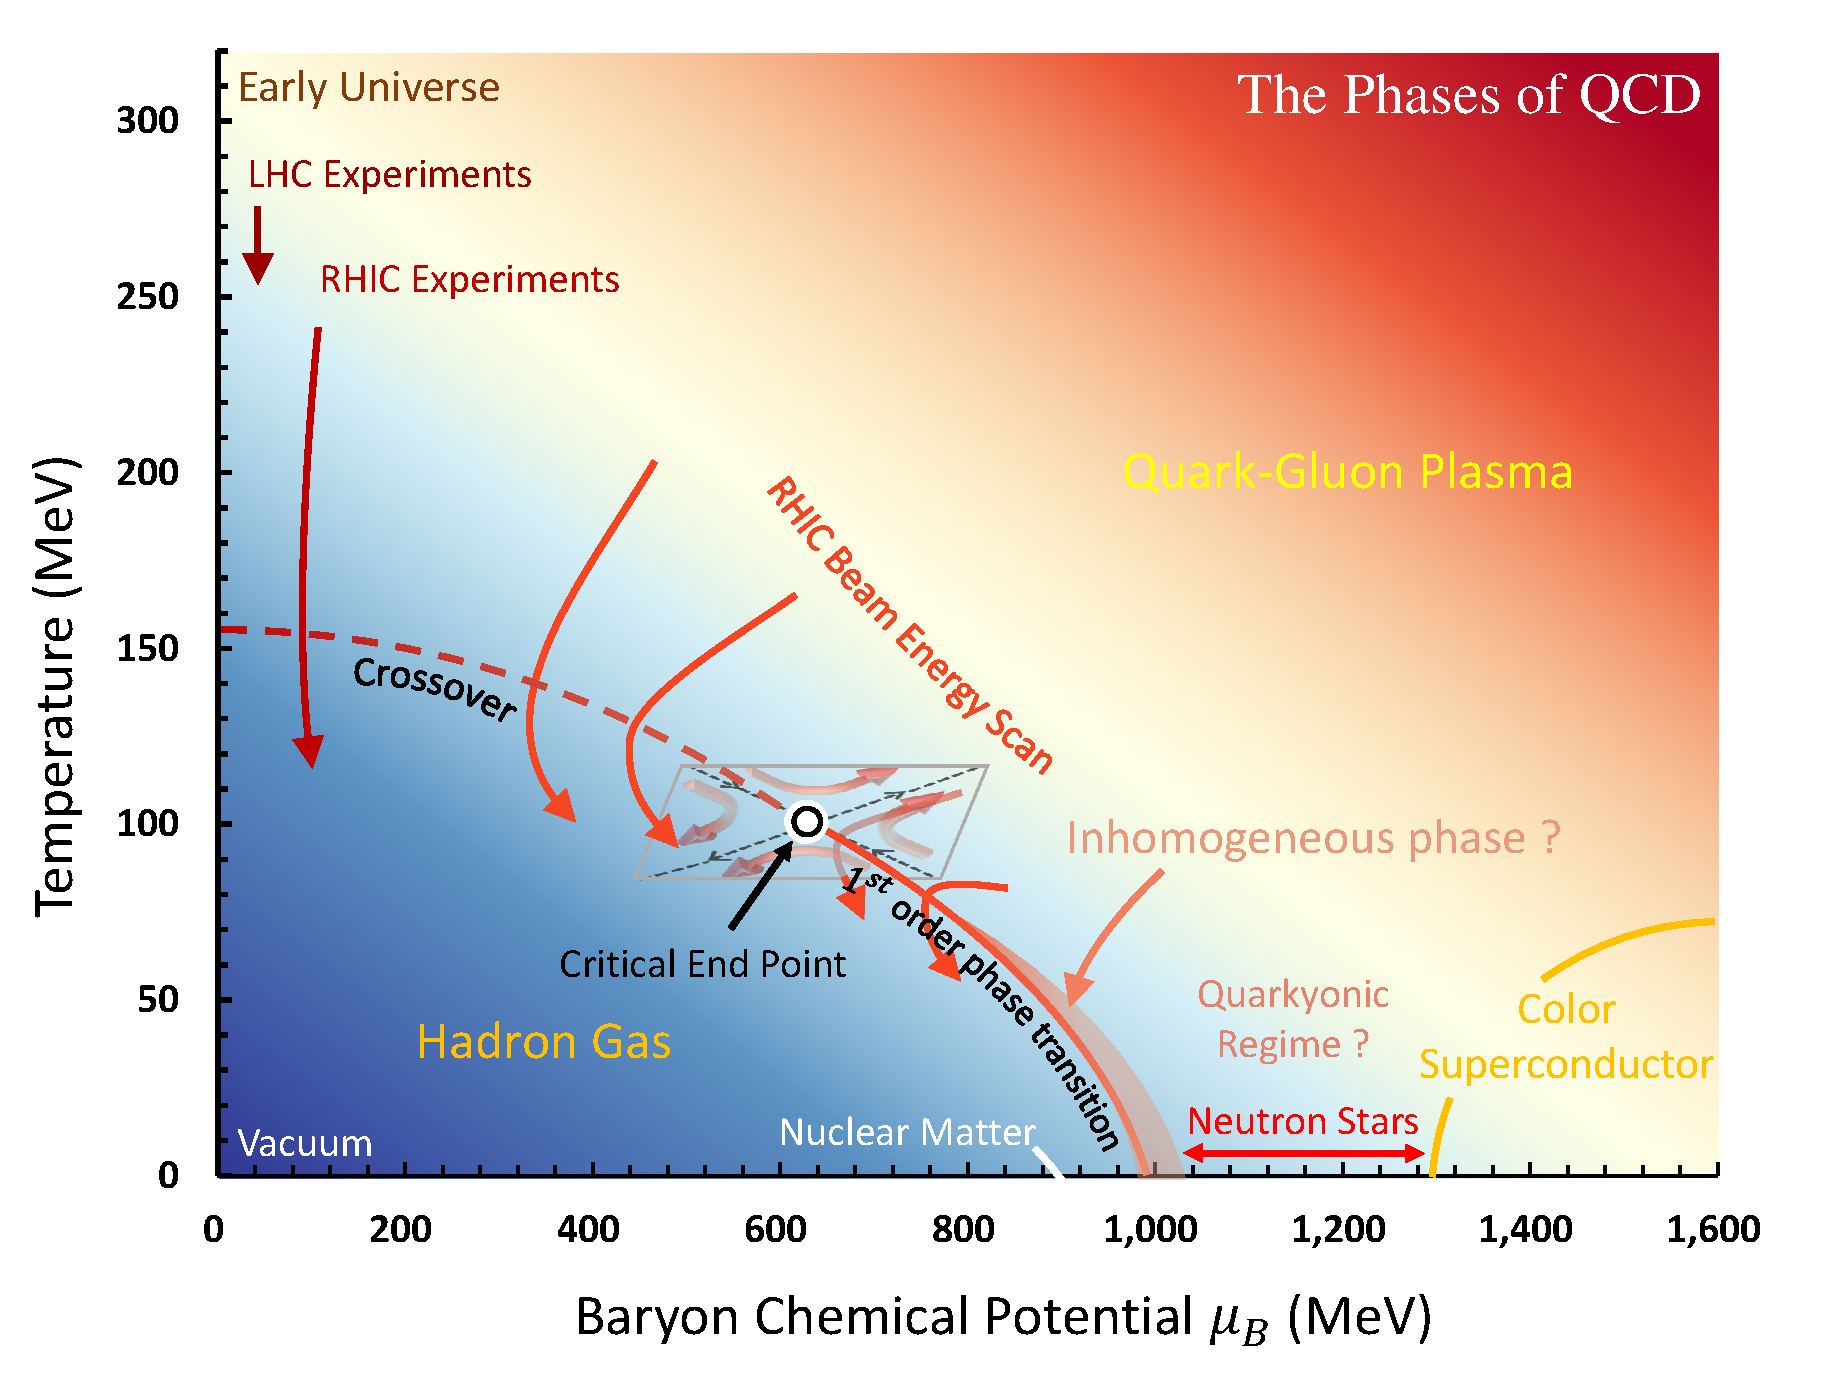
\includegraphics[width=1.15\linewidth]{Images/Figures/chap1_phase20240311.pdf}
            \vspace{-1.cm}
            \hspace{0.7cm}
            \hspace{1cm}{\scriptsize Nucl.Tech. 46 (2023) 04, 040002-040002}
            \vspace{1cm}
        \end{column}
    \end{columns}
\end{frame}
%%%%%%%%%%%%%%%%%%%%%%%%%%%%%%%%%%%%%%%%%%%%%%%%%%%%%%%%%%%%%%%%%%%%%%%%%%%%%
\begin{frame}[fragile]{Theoretical predictions}
    \begin{columns}
        \begin{column}{0.43\textwidth}
            \vspace{-7cm}
            \begin{itemize}
            \item Lattice QCD (at vanishing chemical potential)\\~\
            \item Dyson-Schwinger Equations (DSE)\\~\
            \item Functional renormalization group (fRG)\\~\
            \item ...
            \end{itemize}
        \end{column}
        \begin{column}{0.5\textwidth}
            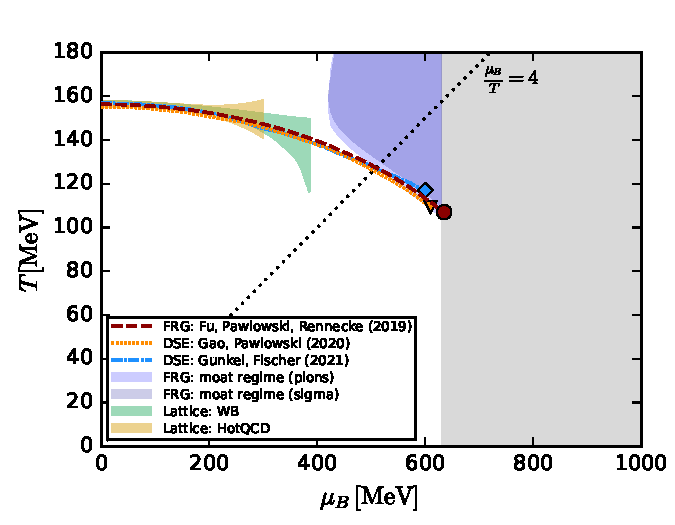
\includegraphics[width=1.15\linewidth]{Images/Figures/phasestructure_v4.pdf}
            \vspace{-0.8cm}
            \hspace{0.7cm}
            \hspace{2cm}{\scriptsize QCD phase diagram (fQCD 2025)}
            \vspace{8cm}
        \end{column}
    \end{columns}
\end{frame}
%%%%%%%%%%%%%%%%%%%%%%%%%%%%%%%%%%%%%%%%%%%%%%%%%%%%%%%%%%%%%%%%%%%%%%%%%%%%%
\begin{frame}[fragile]{Well known Advantages $\&$ Disadvantages}
    \vspace{-0.2cm}
    \begin{columns}
        \begin{column}{0.5\textwidth}
         \vspace{-1.29cm}
         \begin{block}{Lattice:}
            \begin{itemize}
            \item Reliable at 0 chemical potential\\~\
            \item Expansion methods are needed to reach finite density\\~\
            \end{itemize}
         \end{block}
         \vspace{0.8cm}
        \begin{itemize}
        \item Making reasonable use of reliable vanishing chemical potential results\\~\
        \item Attempt to reach higher chemical potentials
        \end{itemize}
        \end{column}
        \begin{column}{0.5\textwidth}
        \begin{block}{Functional methods:}
            \begin{itemize}
            \item Can compute at finite density\\~\
            \item Have to use truncations to prevent an infinite number of loop diagrams \\~\
            \end{itemize}
        \end{block}
        \hspace{0.5cm}
        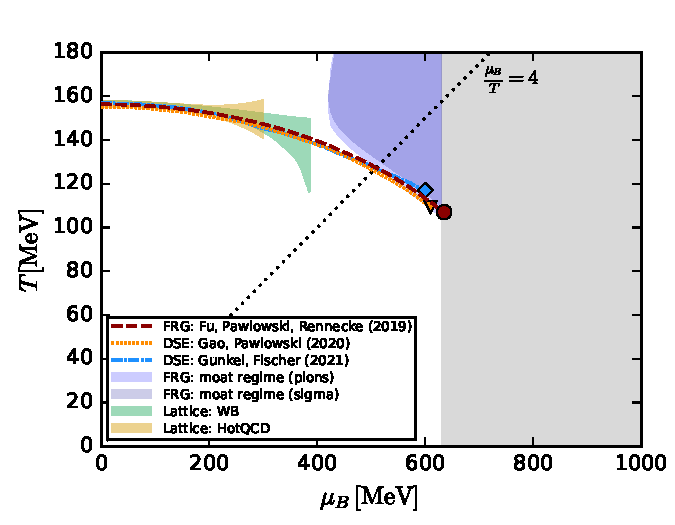
\includegraphics[width=0.82\linewidth]{Images/Figures/phasestructure_v4.pdf}
        \end{column}
    \end{columns}
\end{frame}
%%%%%%%%%%%%%%%%%%%%%%%%%%%%%%%%%%%%%%%%%%%%%%%%%%%%%%%%%%%%%%%%%%%%%%%%%%%%%
\subsection{Extrapolation to finite density}

\begin{frame}[fragile]
    \vspace{-0.2cm}
    \begin{block}{Taylor Expansion of the pressure:}
        \begin{align}
            \frac{p(T,\hat{\mu}_B)-p(T,0)}{T^4}=\sum^{\infty}_{n=1}\frac{1}{(2n)!}\chi^B_{2n}(T,0)\,\hat{\mu}_B^{2n}
        \end{align}
    \end{block}
    HotQCD: \hspace{7cm}WB:
    \vspace{0.5cm}
    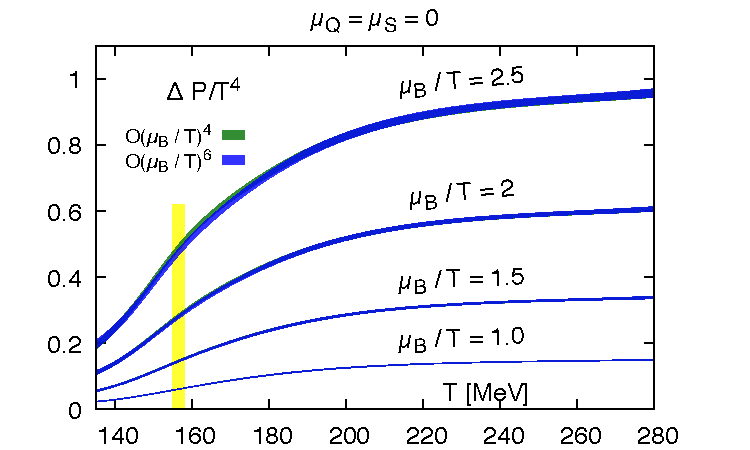
\includegraphics[width=0.5\linewidth,trim={0 0 0 0.6cm}, clip]{Images/Figures/Temp_BQS000_muB_Order_test.pdf}\hspace{1cm}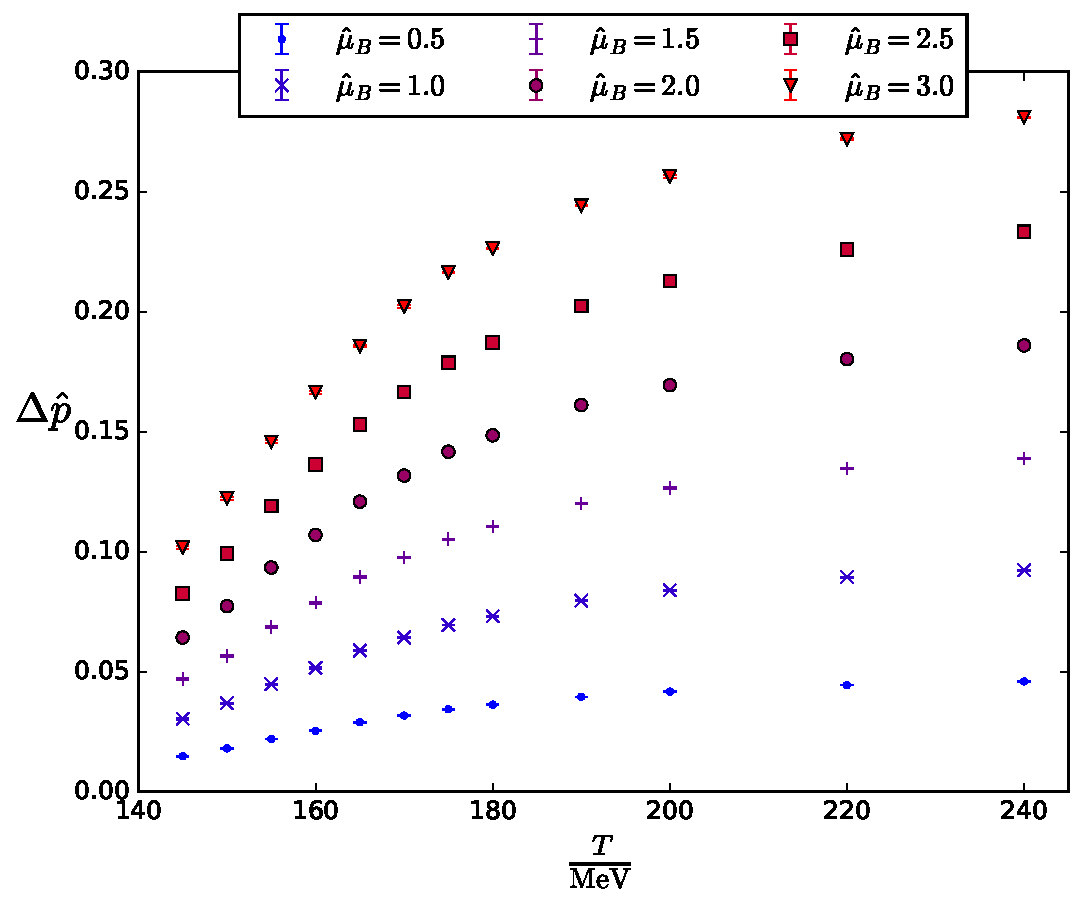
\includegraphics[width=0.4\linewidth,trim={0 1.3cm 0 0}, clip]{Images/Figures/plot6.pdf}
\end{frame}
%%%%%%%%%%%%%%%%%%%%%%%%%%%%%%%%%%%%%%%%%%%%%%%%%%%%%%%%%%%%%%%%%%%%%%%%%%%%%
\begin{frame}[fragile]{Extrapolation to finite density}
    \vspace{-0.2cm}
    \begin{block}{Pad\'{e} approximation:}
        \begin{align}
            P[m,n]=\frac{p(T,\hat{\mu}_B)-p(T,0)}{T^4}=\frac{\sum^{n/2}_{i=1}a_i\,\,\hat{\mu}_B^{2i}}{1+\sum^{m/2}_{j=1}b_i\,\,\hat{\mu}_B^{2j}}
        \end{align}
    \end{block}
    Here the coefficients $a_i$ and $b_i$ are determined by 
    \begin{align}
       \frac{\partial^iP[m,n]}{\partial\hat{\mu}_B^i}=\chi^B_i
    \end{align}
    \begin{itemize}
    \item When $m=0$ the Pad\'{e} approximation will go back to Taylor expansion
    \item The poles of Pad\'{e} approximation can be used to estimate the convergence radius of Taylor expansion
    \end{itemize}
\end{frame}
%%%%%%%%%%%%%%%%%%%%%%%%%%%%%%%%%%%%%%%%%%%%%%%%%%%%%%%%%%%%%%%%%%%%%%%%%%%%%
\begin{frame}[fragile]{Extrapolation to finite density}
    \vspace{-0.2cm}
    \begin{block}{Ratio estimator: (the pole of P[2,n])}
        \begin{align}
            r^{\mathrm{ratio}}_{c,2n}=\bigg| \frac{(2n+1)(2n+2)\chi^B_{2n}}{\chi^B_{2n+2}} \bigg|^{\frac{1}{2}}
        \end{align}
    \end{block}
    \begin{block}{Mercer-Roberts estimator: (the pole of P[4,n])}
    \begin{align}
            r^{\mathrm{MR}}_{c,2n}=&\bigg|\bigg[ \frac{\chi^B_{2n+2}\chi^B_{2n-2}}{(2n+2)!(2n-2)!}-\bigg(\frac{\chi^B_{2n}}{(2n)!}\bigg)^2 \bigg]\bigg|^{\frac{1}{4}}\,\,\bigg|\bigg[ \frac{\chi^B_{2n}\chi^B_{2n+4}}{(2n)!(2n+4)!}-\bigg(\frac{\chi^B_{2n+2}}{(2n+2)!}\bigg)^2 \bigg]\bigg|^{-\frac{1}{4}}
    \end{align}
    \end{block}
    \vspace{0.5cm}
    \begin{itemize}
    \item The estimators are given by the poles of the Pad\'{e} approximation 
    \item They can give a approximation convergence radius of Taylor expansion
    \end{itemize}
\end{frame}
%%%%%%%%%%%%%%%%%%%%%%%%%%%%%%%%%%%%%%%%%%%%%%%%%%%%%%%%%%%%%%%%%%%%%%%%%%%%%
\begin{frame}[fragile]{Extrapolation to finite density}
    \vspace{-0.2cm}
    \begin{block}{T' expansion:}
    \vspace{-0.2cm}
        \begin{align}
            \frac{\chi^B_1(T,\hat{\mu}_B)}{\hat{\mu}_B}&=\chi^B_2(T',0)\\
            T'(T,\hat{\mu}_B)=T\Big(1+\kappa_2(T)&\,\hat{\mu}_B^2+\kappa_4(T)\,\hat{\mu}_B^4+\mathcal{O}(\hat{\mu}_B^6)\Big)
        \end{align}
    \end{block}
    \vspace{0cm}
    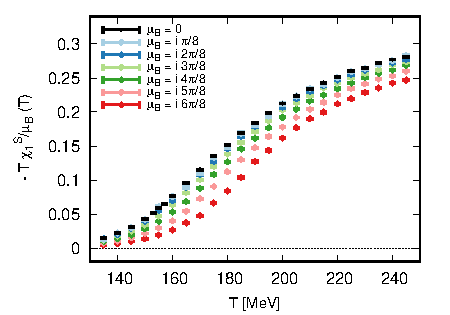
\includegraphics[width=0.47\linewidth,trim={0 0 0 0.28cm}, clip]{Images/Figures/shift_48x12_BS.pdf}\hspace{0.5cm}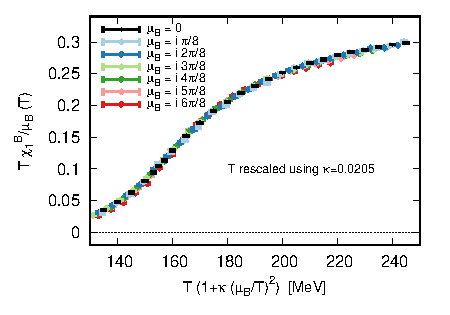
\includegraphics[width=0.48\linewidth,trim={0 0 0 0}, clip]{Images/Figures/shift_48x12_B2_collapse.pdf}\\
    \vspace{-0.3cm}{\centering \scriptsize Phys. Rev. Lett. 126, 232001 (2021) \par}
\end{frame}
%%%%%%%%%%%%%%%%%%%%%%%%%%%%%%%%%%%%%%%%%%%%%%%%%%%%%%%%%%%%%%%%%%%%%%%%%%%%%
% Remember to input this to the presentative tex file before compiling.
\section{EoS from fRG}

\subsection{Polyakov-Quark-Meson (PQM) Model}

\begin{frame}
\begin{block}{Effective action:}
    \begin{align}
     \Gamma_k=&\int_x \Big\{ Z_q\,\bar{q}\big[\gamma_\mu\partial_\mu-\gamma_0(\mu+igA_0)\big]q+\frac{1}{2}Z_\phi\,(\partial_\mu\phi)^2 \nonumber\\
     &+h\,\bar{q}(T^0\sigma+i\gamma_5\vec{T}\cdot\vec{\pi})+V_k(\rho)-c\sigma+V_{\mathrm{glue}}(L,\bar{L}) \Big\}
    \end{align}
\end{block}

Here we use Local potential approximation (LPA):
\begin{align}
&\partial_tZ_{q/\phi}=0\\[2ex]
&\partial_th=0
\end{align}
We only consider a simple computation of the Grand potential.
\end{frame}
%%%%%%%%%%%%%%%%%%%%%%%%%%%%%%%%%%%%%%%%%%%%%%%%%%%%%%%%%%%%%%%%%%%%%%%%%%%%
\begin{frame}[fragile]{Effective potential}
\begin{block}{Flow equation of effective potential:}
    \begin{align}
     \partial_t V_k(\rho)=\frac{k^4}{4\pi^2}\Bigg[3\,l^{(B)}_0(m^2_\pi; T)+l^{(B)}_0(m^2_\sigma; T)-4N_cN_fl^{(F)}_0(m^2_f;\mu, T)\Bigg]
    \end{align}
\end{block}
The fermion loop for real and imaginary chemical potential
\begin{align}
    l^{(F)}_0(m^2_f;\mu, T)&=\frac{k}{3\sqrt{k^2+m^2_f}}\bigg(1-n_F(m^2_f;\mu, T;L,\bar{L})-\bar{n}_F(m^2_f;-\mu, T;L,\bar{L})\bigg)\\
    &=\frac{k}{3\sqrt{k^2+m^2_f}}\bigg(1-2\,\,\mathrm{Re}\Big(n_F(m^2_f;\mu, T;L,\bar{L})\Big)\bigg)
\end{align}
\end{frame}
%%%%%%%%%%%%%%%%%%%%%%%%%%%%%%%%%%%%%%%%%%%%%%%%%%%%%%%%%%%%%%%%%%%%%%%%%%%%
\begin{frame}[fragile]{Equation of State}
%\begin{enumerate}
    \begin{columns}
        \begin{column}{0.5\textwidth}
           \vspace{-6.5cm}
           \begin{block}{Pressure and Baryon number fluctuations:}
           \begin{align}
                p(T,\mu)=&-\Omega(\mu,T)\\[2ex]
                \chi^B_n=\frac{\partial^n}{\partial\hat{\mu}_B^n}\frac{p}{T^4},&\qquad \hat{\mu}_B=\frac{\mu_B}{T}\\[2ex]
                R^B_{m,n}=&\frac{\chi^B_m}{\chi^B_n}
           \end{align}
           \end{block}
           \hspace{0.8cm}
           \begin{itemize}
           \item The baryon number fluctuations at vanishing chemical potential can be used as Taylor coefficients
           \end{itemize}
        \end{column}
        \begin{column}{0.5\textwidth}
            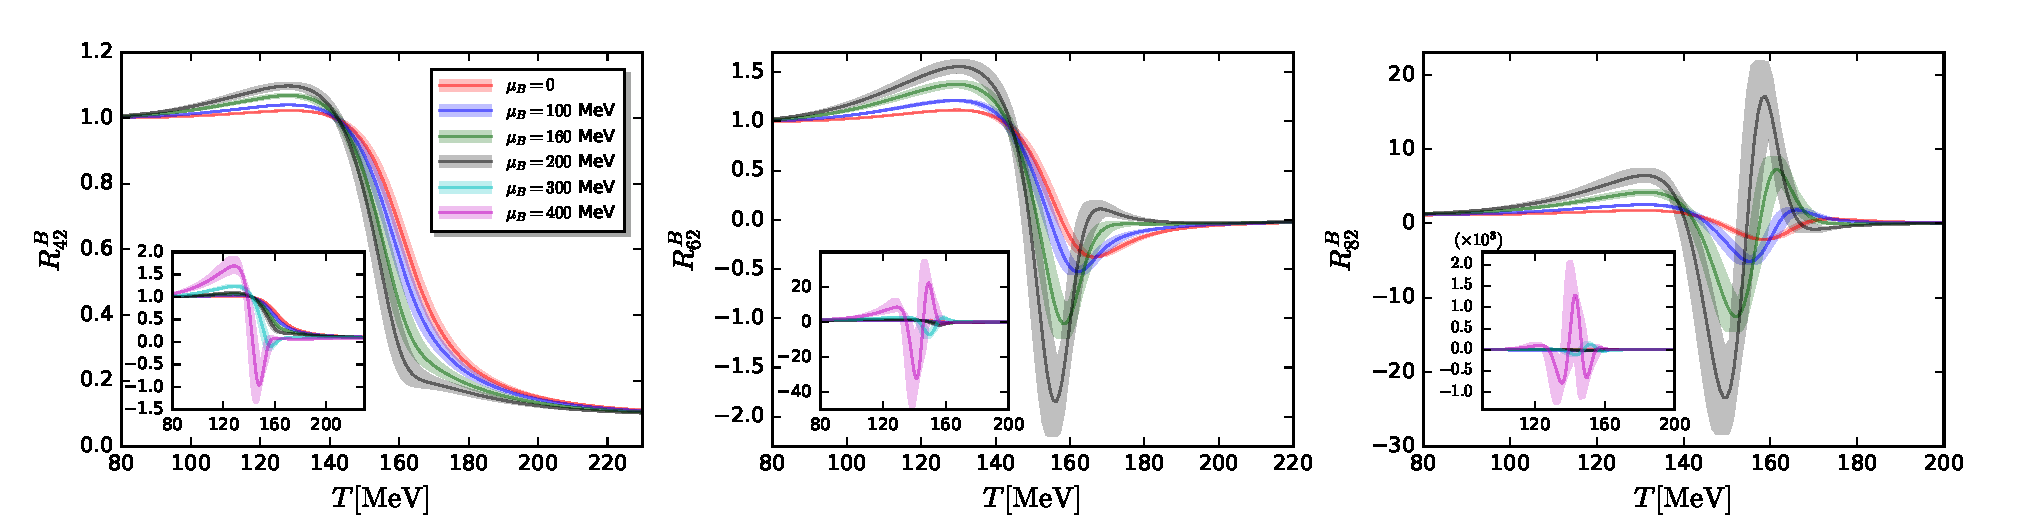
\includegraphics[width=1.\linewidth,trim={0 0 23cm 0}, clip]{Images/Figures/R42R62R82-T-muB0to400.pdf}
            \vspace{-0.8cm}
            %\hspace{0.7cm}
            \hspace{2cm}{\scriptsize Phys.Rev.D 104 (2021) 9, 094047}            
            \vspace{8cm}
        \end{column}
    \end{columns}
%\end{enumerate}
\end{frame}
%%%%%%%%%%%%%%%%%%%%%%%%%%%%%%%%%%%%%%%%%%%%%%%%%%%%%%%%%%%%%%%%%%%%%%%%%%%%
\begin{frame}[fragile]{Equation of State}
    \begin{columns}
        \begin{column}{0.5\textwidth}
           \begin{itemize}
           \item The baryon number fluctuations can be computed up to (at least) the 10th order
           \end{itemize}
        \end{column}
        \begin{column}{0.5\textwidth}
            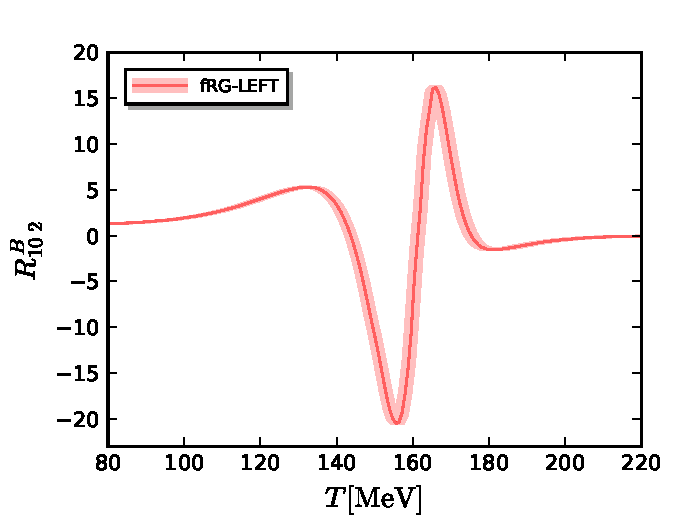
\includegraphics[width=1.\linewidth]{Images/Figures/R102-T-muB0.pdf}
            \vspace{-0.8cm}
            %\hspace{0.7cm}
            \hspace{2cm}{\scriptsize Phys.Rev.D 104 (2021) 9, 094047}            
            %\vspace{8cm}
        \end{column}
    \end{columns}
\end{frame}
%%%%%%%%%%%%%%%%%%%%%%%%%%%%%%%%%%%%%%%%%%%%%%%%%%%%%%%%%%%%%%%%%%%%%%%%%%%%
\subsection{Comparison of different Expansion methods}

\begin{frame}[fragile]
    Taylor Expansion
    \centering
    \vspace{-0.3cm}
    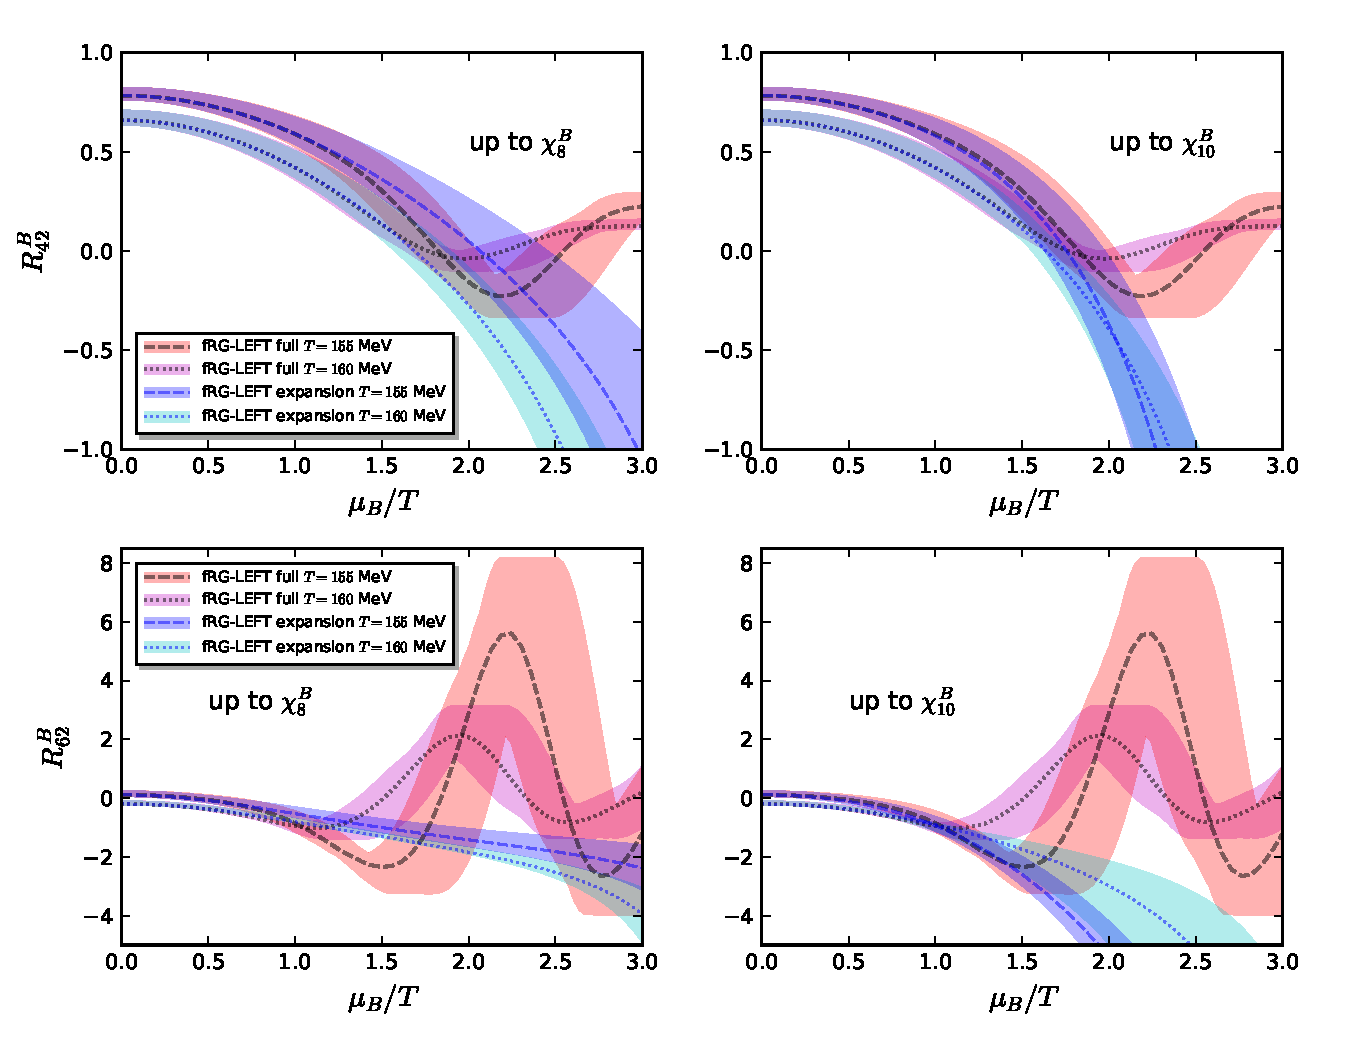
\includegraphics[width=0.9\linewidth,trim={0 9cm 0 0.5cm}, clip]{Images/Figures/R42R62expansion-muBoT.pdf}\\
    {\scriptsize Phys.Rev.D 104 (2021) 9, 094047}
    \begin{itemize}
    \item Direct calculation vs. Taylor expansion of $R^B_{42}$ \\~\
    \item The $R^B_{42}$ around $T_{pc}$ exhibits strong fluctuations at high chemical potential, which are difficult to capture with a finite-order Taylor expansion.
    \end{itemize}  
\end{frame}
%%%%%%%%%%%%%%%%%%%%%%%%%%%%%%%%%%%%%%%%%%%%%%%%%%%%%%%%%%%%%%%%%%%%%%%%%%%%
\begin{frame}[fragile]{Comparison of different Expansion methods}
    \centering
    T' Expansion
    \vspace{-0.1cm}
    \begin{columns}
        \begin{column}{0.5\textwidth}
            \includegraphics[width=0.9\linewidth]{Images/Figures/chi1_mub.pdf}
        \end{column}
        \begin{column}{0.5\textwidth}
            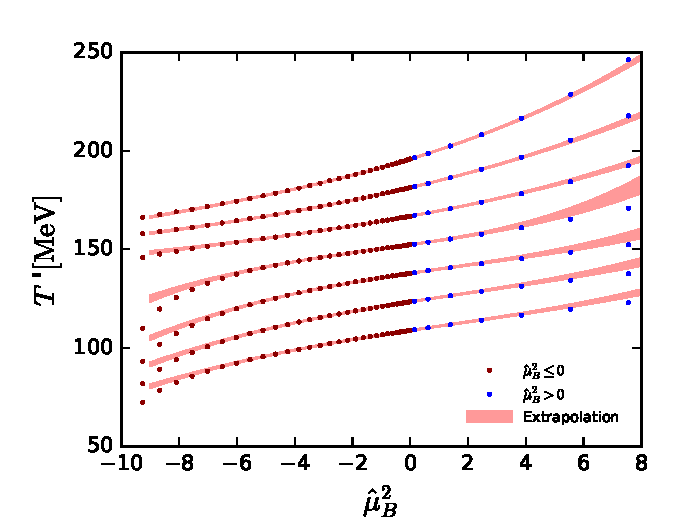
\includegraphics[width=0.9\linewidth]{Images/Figures/Ext.pdf}
        \end{column}
    \end{columns}
    {\centering \scriptsize arXiv: 2403.06770 \par}
    \begin{itemize}
    \item Directly compute at imaginary chemical potential 
    \item Apply the T’ expansion to perform extrapolation
    \end{itemize} 
\end{frame}
%%%%%%%%%%%%%%%%%%%%%%%%%%%%%%%%%%%%%%%%%%%%%%%%%%%%%%%%%%%%%%%%%%%%%%%%%%%%
\begin{frame}[fragile]{Comparison of different Expansion methods}
    \centering
    T' Expansion\\
    \vspace{-0.1cm}
    \begin{columns}
        \begin{column}{0.5\textwidth}
            \begin{align}
              T'=T\bigg( 1&+\kappa^B_2(T)\,\hat{\mu}_B^2+\kappa^B_4(T)\,\hat{\mu}_B^4\nonumber\\[2ex]
              &+\kappa^B_6(T)\,\hat{\mu}_B^6+\cdots \bigg)
            \end{align}
        \end{column}
        \begin{column}{0.5\textwidth}
            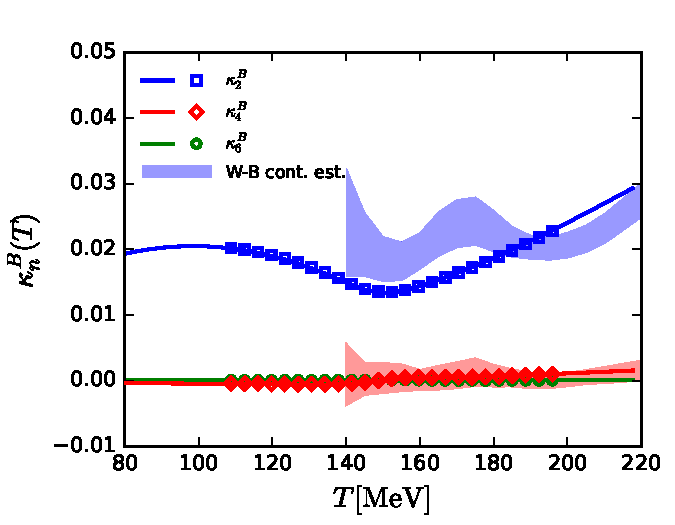
\includegraphics[width=1.\linewidth]{Images/Figures/kappa.pdf}
           {\centering \scriptsize arXiv: 2403.06770 \par}
        \end{column}
    \end{columns}
\end{frame}
%%%%%%%%%%%%%%%%%%%%%%%%%%%%%%%%%%%%%%%%%%%%%%%%%%%%%%%%%%%%%%%%%%%%%%%%%%%%
\begin{frame}[fragile]{Comparison of different Expansion methods}
    \centering
    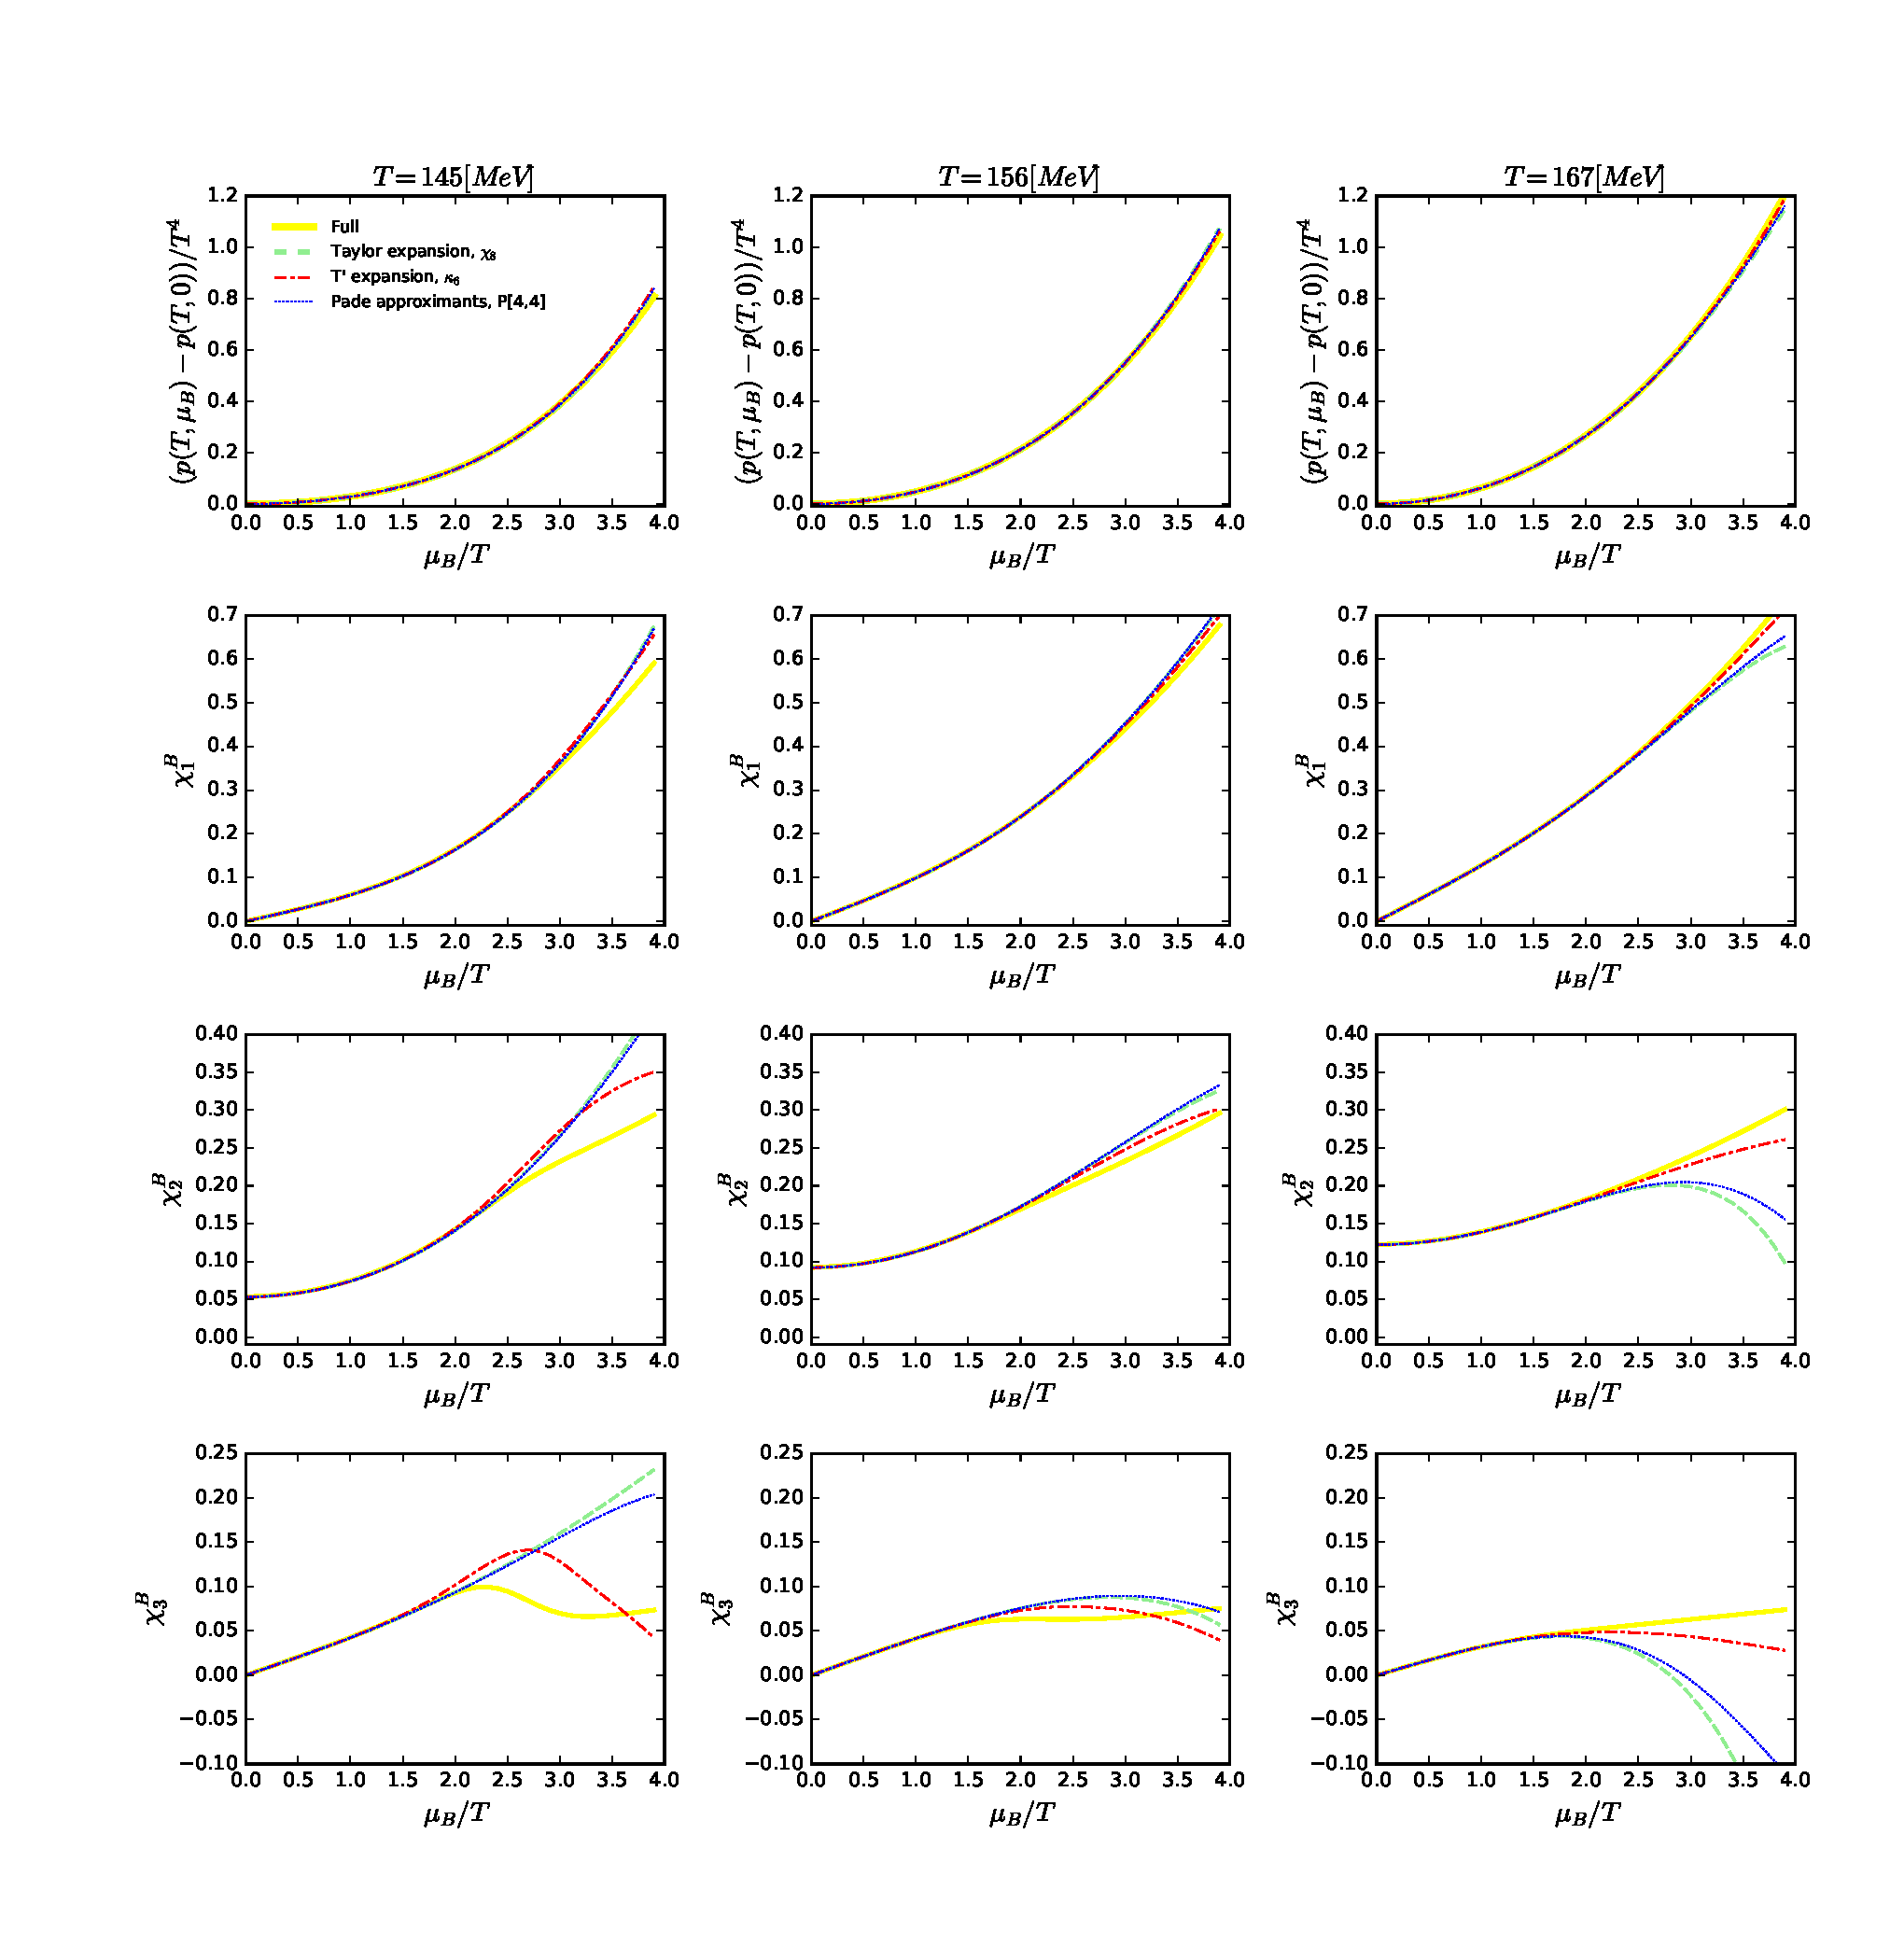
\includegraphics[width=1.\linewidth,trim={2cm 17cm 0 2.9cm}, clip]{Images/Figures/FixT.pdf}
    {\centering \scriptsize arXiv: 2403.06770 \par}
\end{frame}
%%%%%%%%%%%%%%%%%%%%%%%%%%%%%%%%%%%%%%%%%%%%%%%%%%%%%%%%%%%%%%%%%%%%%%%%%%%%
\begin{frame}[fragile]{Comparison of different Expansion methods}
    \centering
    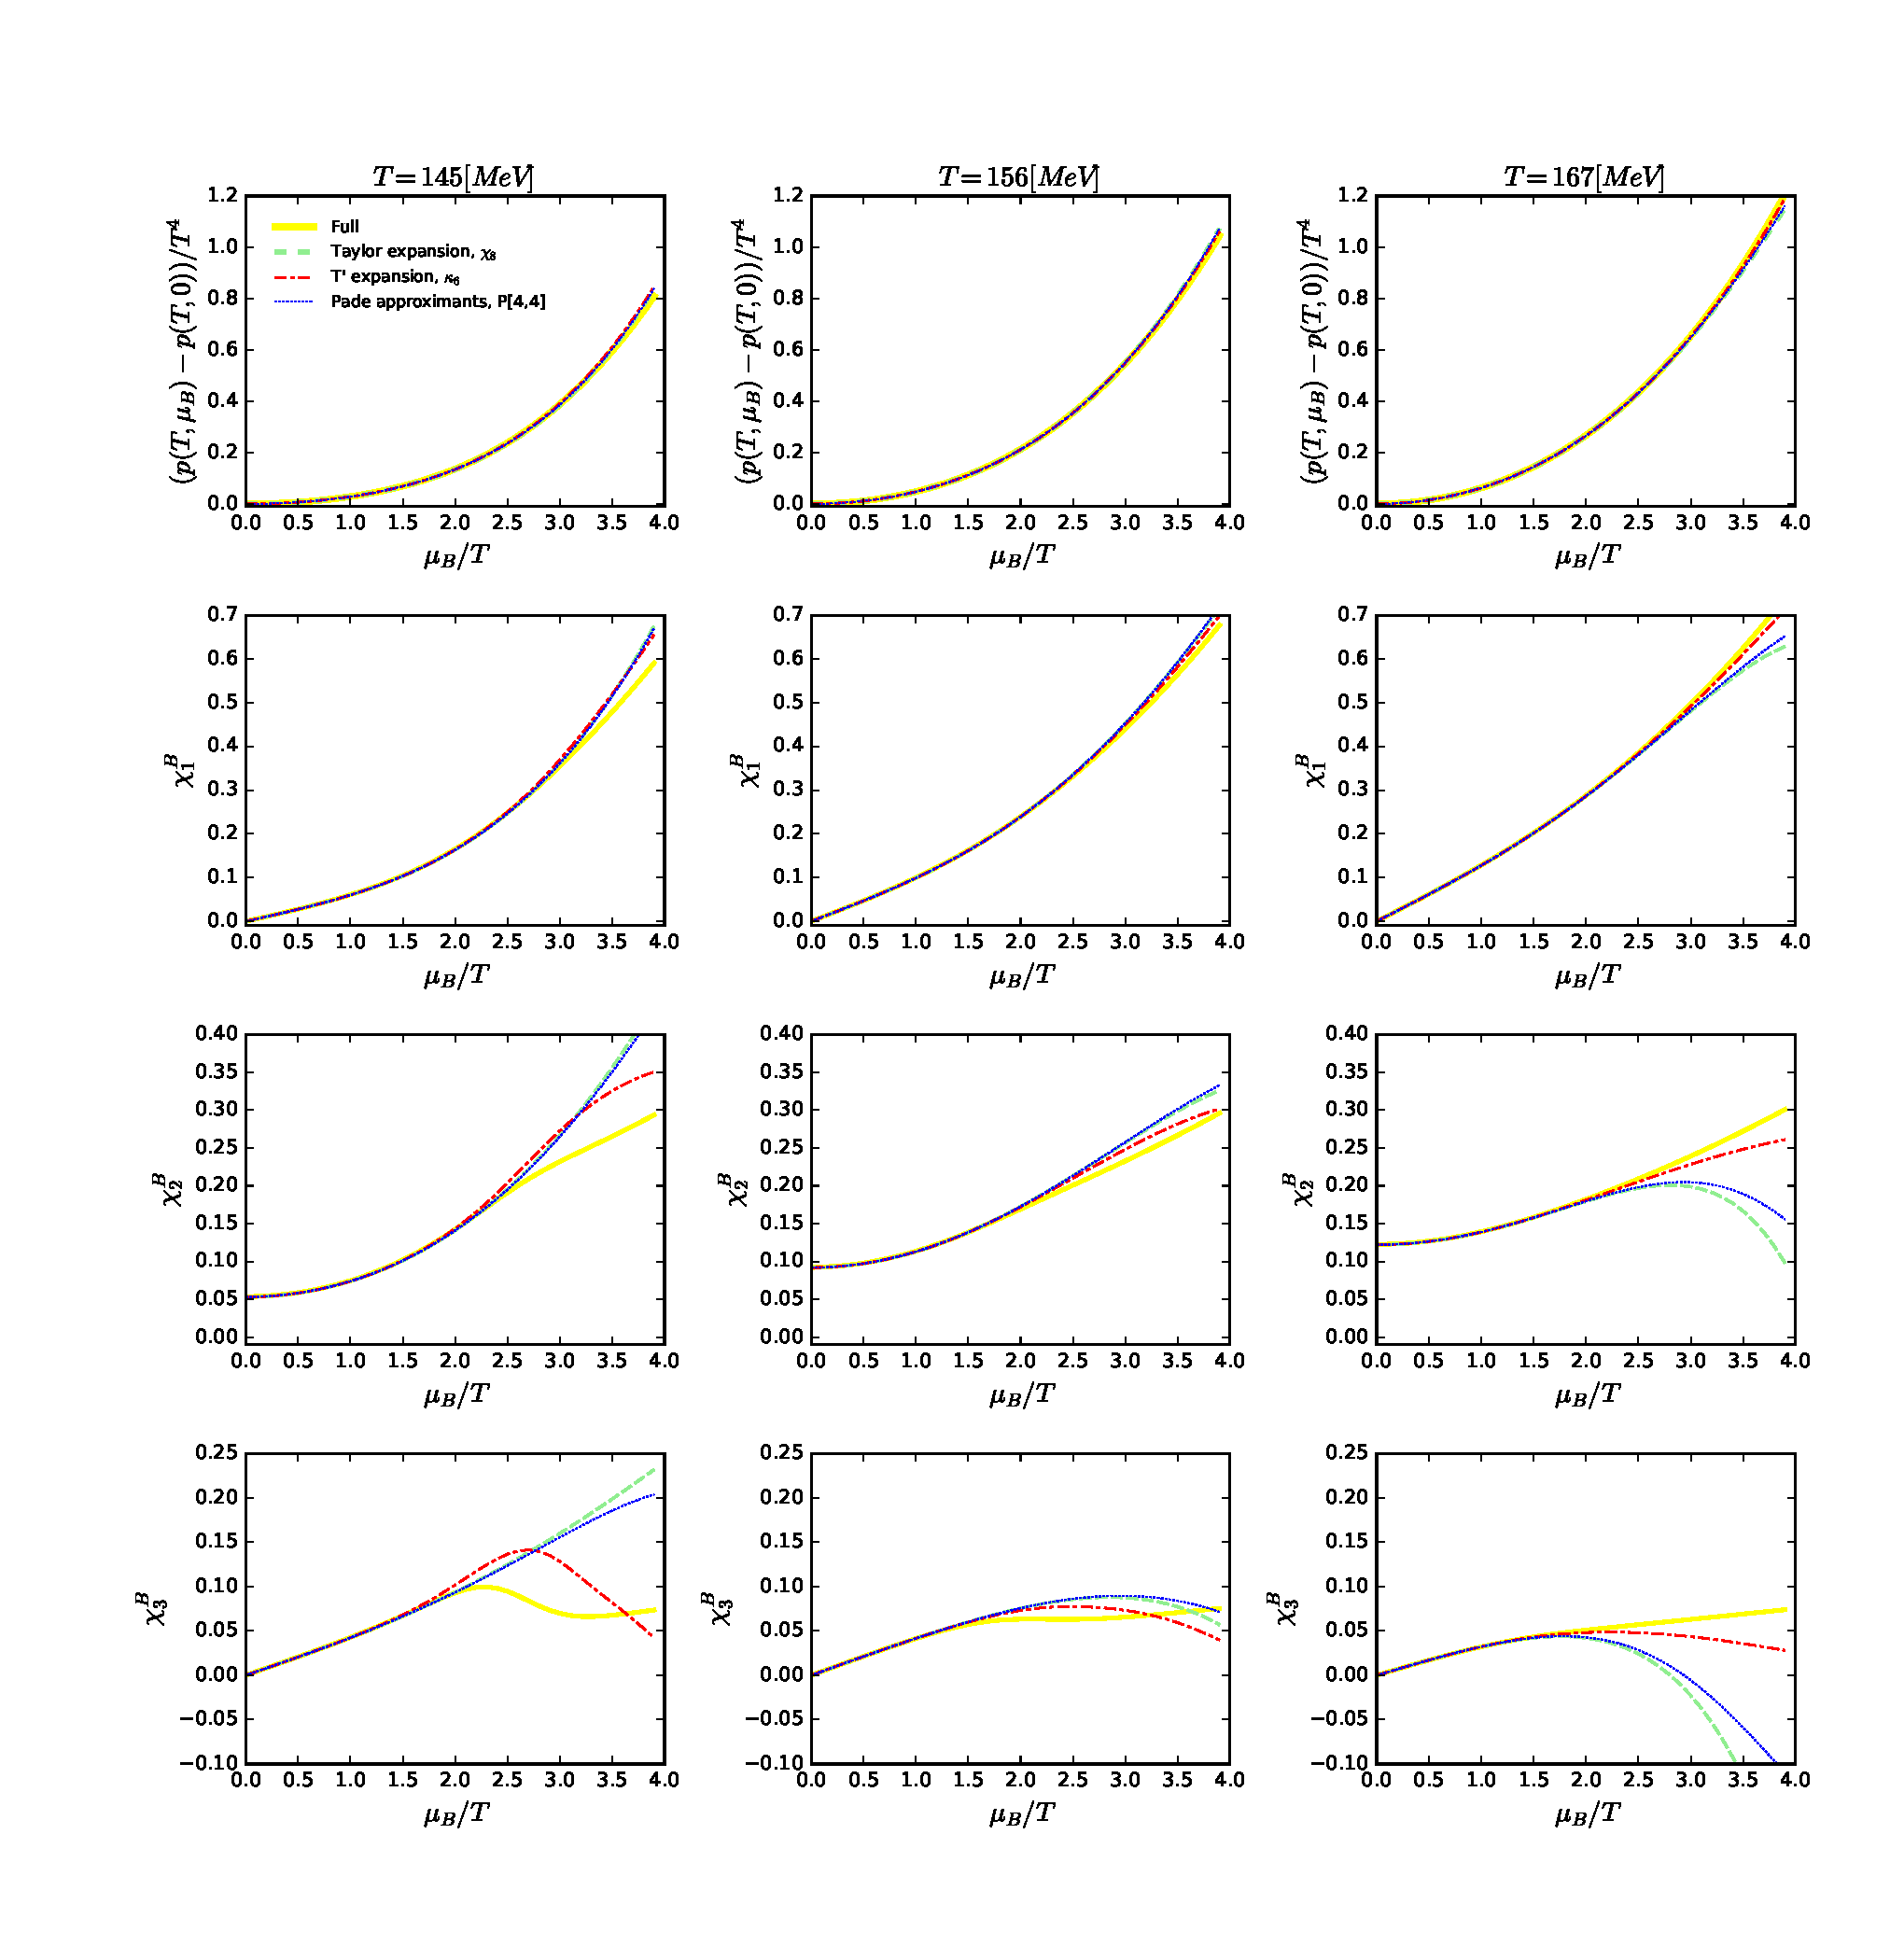
\includegraphics[width=1.\linewidth,trim={2cm 2cm 0 18cm}, clip]{Images/Figures/FixT.pdf}
    {\centering \scriptsize arXiv: 2403.06770 \par}
\end{frame}
%%%%%%%%%%%%%%%%%%%%%%%%%%%%%%%%%%%%%%%%%%%%%%%%%%%%%%%%%%%%%%%%%%%%%%%%%%%%
\begin{frame}[fragile]{Comparison of different Expansion methods}
    \centering
    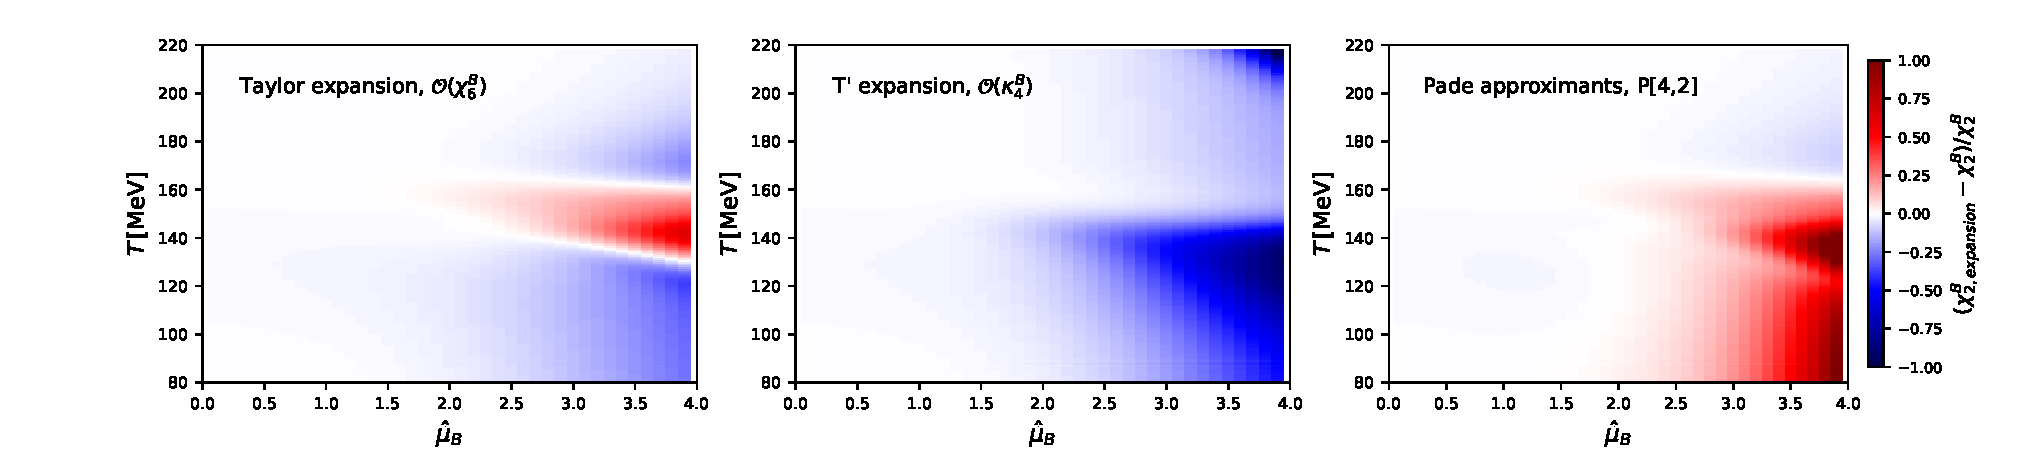
\includegraphics[width=0.87\linewidth,trim={0 0.7cm 0 0.6cm}, clip]{Images/Figures/diffchi2_3A.pdf}\\
    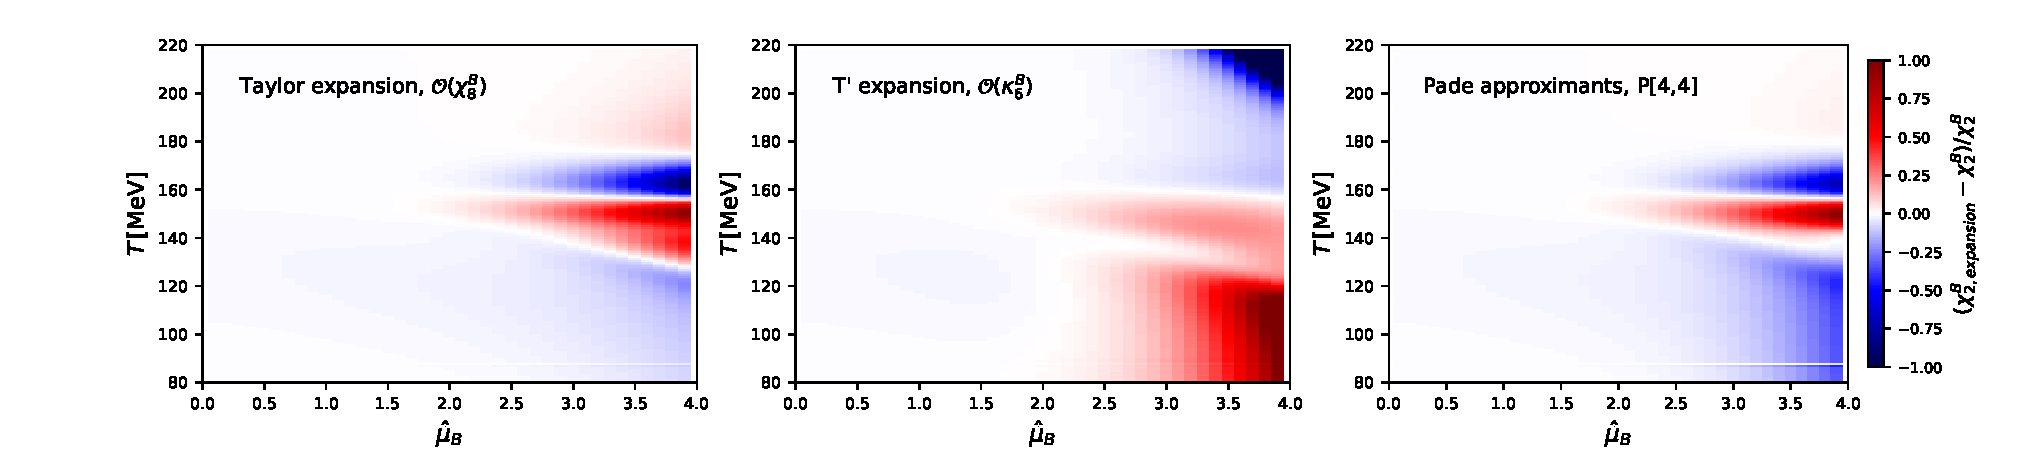
\includegraphics[width=0.87\linewidth,trim={0 0.7cm 0 0.6cm}, clip]{Images/Figures/diffchi2_3.pdf}\\
    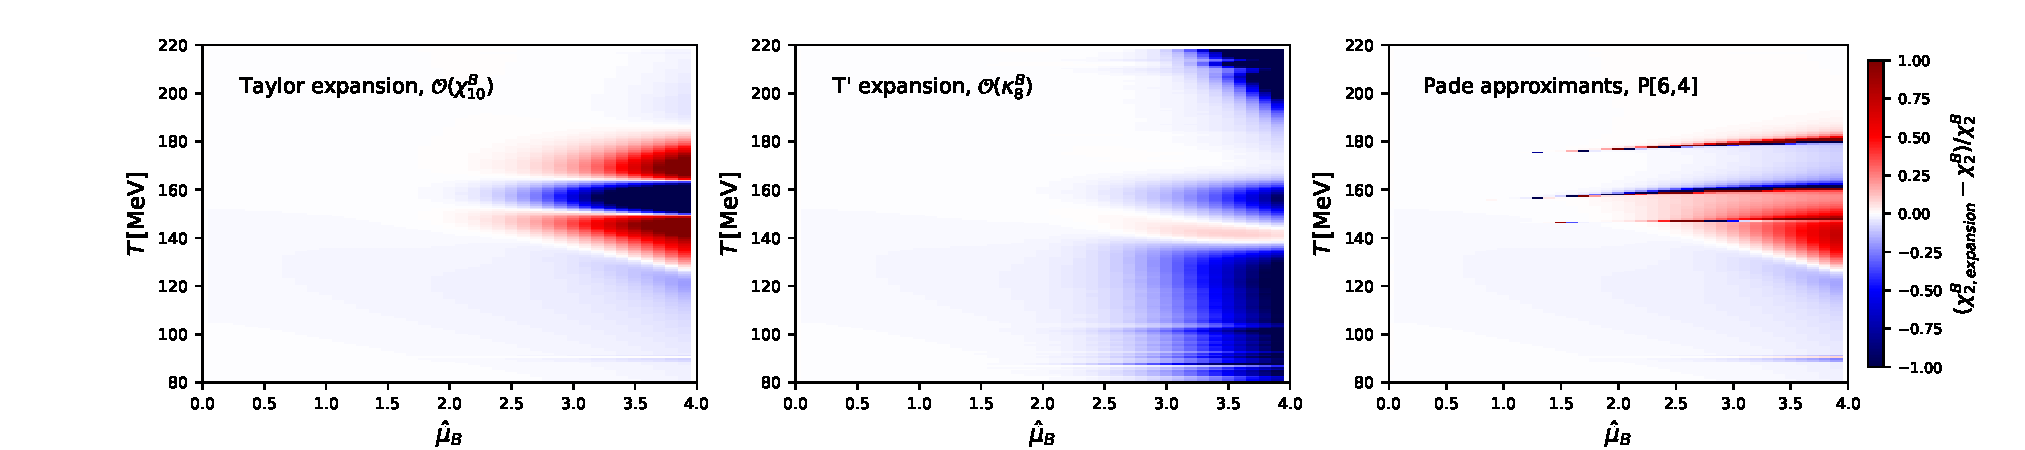
\includegraphics[width=0.87\linewidth,trim={0 0 0 0.6cm}, clip]{Images/Figures/diffchi2_3B.pdf}\\
    {\centering \scriptsize arXiv: 2403.06770 \par}
\end{frame}
%% Remember to input this to the presentative tex file before compiling.
\section{Summary}
\begin{frame}
    \uncover<1->{\Large Mention your findings here.}
    \par~\\\
    \uncover<2->{\Huge Happy \TeX ing!}
\end{frame}
%\section{Summing Up}

% This section is a placeholder to review crucial points to take away from your presentation.



\begin{frame}{Q\&A}
\begin{center}
{\Huge Thank You!}\\[10pt]
I will now be taking questions.
\end{center}
\end{frame}

% References
\begin{frame}[allowframebreaks]
    \frametitle{References}
    \nocite{*}
    \printbibliography
\end{frame}

% Appendix
\appendix
% The appendix tex file gets inputted after the /appendix command in the main tex file.
% Treat your appendices as you would regular chapters, sections and subsections, and they would be automatically discounted as appendices.

\section{Appendix I} \label{app1}
%\subsection{Appendix 1.1 Scenario 1}
%\subsection{Appendix 1.2 Scenario 2}
\begin{frame}
{\Large Appendix I: Title}
    \begin{remark}
    This is what an appendix would look like. It utilises the same structure as the rest of the presentation \textit{(section, subsection, subsubsection, etc)}.
    \end{remark}
    \begin{exampleblock}{Example}
    \textcolor{mygrey}{\lipsum[2][1-20]}
    \end{exampleblock}
\end{frame}

\section{Appendix II} \label{app2}
\begin{frame}
{\Large Appendix II: Title} 
    \begin{block}{Relevant Title}
    \textcolor{mygrey}{\lipsum[2][1]}
    \end{block}
    \begin{exampleblock}{Example of Appendix II}
    \textcolor{mygrey}{\lipsum[4][1-20]}
    \end{exampleblock}
\end{frame}

\end{document}
